\section{Umsetzung}
\subsection{Überblick}
Genau wie bei Bitcoin besteht die Möglichkeit die Glücksspielanwendung entweder mithilfe eines \textit{Light Nodes} direkt, oder über einen \textit{Full Node} indirekt, mit dem Ethereum Netzwerk kommunizieren zu lassen. Für den Ethereum Teil dieser Masterarbeit findet die Kommunikation indirekt über einen Full Node statt. Dies ist in Abbildung \ref{fig:eth_anwendung_aufbau} verdeutlicht. Der Full Node empfängt Transaktionen und Blöcke, validiert diese und akualisiert kontinuierlich den Zusatnd der durch die Transaktionen veränderten Ethereum Accounts. Über die RPC Schnittstelle stellt er diese Daten nach außen bereit. Die Java Bibliothek Web3J \cite{web3j} erleichtert den Aufruf der RPC Schnittstelle des Full Nodes. Anders als bei Bitcoin benötigt die Glücksspielanwendung keine eigene Datenbank, da der Zustand des aktuellen Topfs im Smart Contracts und somit ''in der Blockchain'' gespeichert ist.
\begin{figure}[H]
\centering
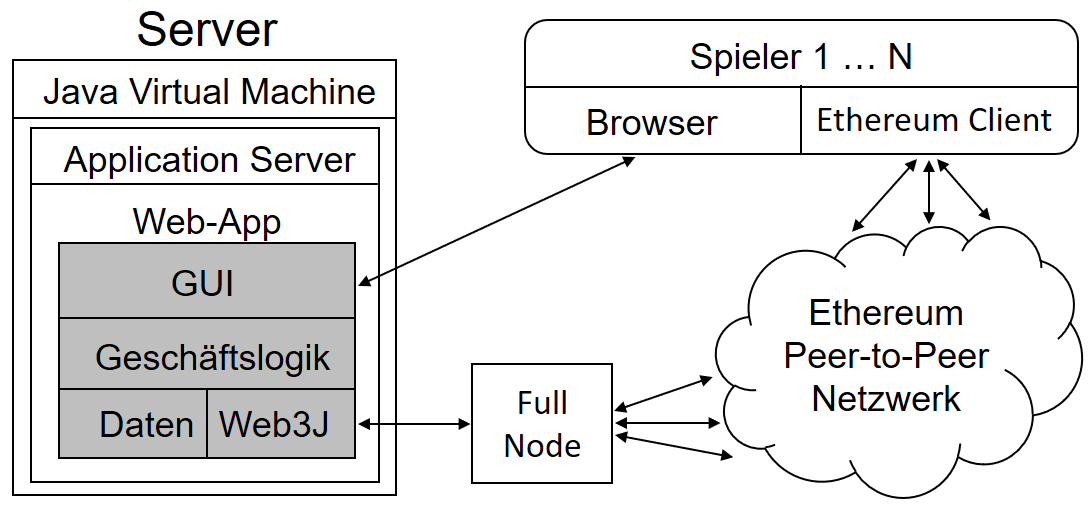
\includegraphics[width=1\linewidth]{Figures/umsetzung_eth/anwendung_aufbau}
\decoRule
\caption{Ethereum: Netzwerk Integration}
\label{fig:eth_anwendung_aufbau}
\end{figure}

Möchte man eine Anwendung direkt in das Ethereum Netzwerk integrieren, bietet sich in Java die Bibliothek EthereumJ \cite{ethereumj} an. 

\subsection{Smart Contract}
Die folgenden Codestücke beschreiben den \code{TrustlessGambling} Smart Contract in der Programmiersprache Solidity\footnote{\url{https://solidity.readthedocs.io/en/v0.4.0/}}.

\subsubsection{Datenmodell}
Das folgenden Codestücke zeigt den Rahmen, alle Variablen und den Konstruktor des Smart Contracts.
\begin{lstlisting}[basicstyle=\small]
pragma solidity ^0.4.0;
contract TrustlessGambling {
    // constants
    uint8 public constant NBR_OF_SLOTS =3;
    uint public constant EXPECTED_POT_AMOUNT=1000;// WEI
    uint8 public constant PAYOUT_BLOCK_OFFSET =1;    
    // pot values
    uint public nbrOfParticipants;
    address[NBR_OF_SLOTS] public depositAddresses;
    address[NBR_OF_SLOTS] public payoutAddresses;
    uint public closingBlockNumber;
    uint public payoutBlockNumber;
    bytes32 public payoutBlockHash;
    uint public winner; // 0 -> NBR_OF_SLOTS-1
    bool public potClosed;
    uint public nbrOfMissedPayouts;
    // constructor
    function TrustlessGambling() public {
        nbrOfParticipants = 0;
        potClosed = false;
        nbrOfMissedPayouts = 0;
    }
}
\end{lstlisting}


Zeile 1 definiert in welcher Version der Solidity Programmiersprache der Smart Contract geschrieben ist. Dies muss vom Compiler bei der Übersetzung zu Bytecode berücksichtigt werden. Zeile 2 legt den Namen des Smart Contracts fest. Über die beiden Konstanten in Zeile 4 und 5 kann man die Anzahl Spieler, und den von jedem Spieler erwarteten Einzahlungsbetrag festlegen. Die in Zeile 6 festgelegte Konstante legt fest, welcher Block ab der letzten Einzahlungstransaktion den Gewinner festlegt. Diese Werte können nach der Bereitstellung des Smart Contracts nicht mehr verändert werden. Die Variablen von Zeile 8 bis Zeile 16 werden vom Smart Contract manipuliert und speichern den Zustand des aktuellen Topfes. Zeile 8 speichert wie viele Teilnehmer bereits eingezahlt haben. Zeile 9 und 10 speichern die Ein- und Auszahlungsadressen\footnote{Die Einzahlungsadressen werden nur zur Anzeige für die GUI-Anwendung abgespeichert und sind für das eigentliche Spiel irrelevant. Das weglassen dieser würde zu günstigeren Transaktionskosten für Einzahlungstransaktionen führen.} der aktuellen Teilnehmer. Die Zeilen 11 bis 14 speichern alle für die Gewinnerauswahl benötigten Werte. Zeile 15 definiert über den Wahrheitswert \code{potClosed}, ob der Topf offen ist und Einzahlungen stattfinden können, oder ob der Topf geschlossen ist. Der Nutzen des Wertes aus Zeile 16 wird im Rahmen des ''Auszahlungen'' Abschnitts erklärt. Zeile 18 bis 22 beinhalten den einmalig bei der Bereitstellung des Smart Contracts aufgerufenen Konstruktor. Alle Variablen des Smart Contracts sind zur Schaffung maximaler Transparenz mit dem Schlüsselwort \code{public} markiert. Dies erlaubt es den Nutzern, alle Werte des Smart Contract abzurufen.

\subsubsection{Einzahlungen}
Einzahlungen finden über die beiden \code{deposit} Methoden statt. Diese sind mit dem Schlüsselwort \code{payable} markiert. Dies bedeutet, dass Transaktionen einen Ether-Betrag beim aufruf dieser Methoden angeben können.
\begin{lstlisting}
function deposit() payable public {
    deposit(msg.sender);
}
function deposit(address _payout) payable public {
    assert(msg.value == EXPECTED_POT_AMOUNT);
    assert(!potClosed);
    depositAddresses[nbrOfParticipants] = msg.sender;
    payoutAddresses[nbrOfParticipants] = _payout;
    nbrOfParticipants++;
    if (nbrOfParticipants == NBR_OF_SLOTS){
        closingBlockNumber = block.number;
        payoutBlockNumber = closingBlockNumber + PAYOUT_BLOCK_OFFSET;
        potClosed = true;
    }
}
\end{lstlisting}


Nutzt der Spieler die Methode aus Zeile 1, wir als Auszahlungsadresse einfach die Adresse der Transaktion verwendet. Nutzt der Spieler die Methode aus Zeile 4, hat er die Möglichkeit eine beliebige Auszahlungsadresse anzugeben. Bei der Einzahlung wird zunächst in Zeile 5 geprüft, ob der der Topf offen ist. Ist dies der Fall, prüft Zeile 6, dass der Transaktionsbetrag mit dem erwarteten Einzahlungsbetrag übereinstimmt. Anschließend werden die Ein- und Auszahlungsadresse abgespeichert und die aktuelle Anzahl Teilnehmer um eins erhöht. Zeile 10 prüft, ob es sich um die letzte Einzahlungstransaktion handelt und schließt den Topf gegebenenfalls. Bevor der Topf geschlossen wird, wird in Zeile 11 die aktuelle Blocknummer abgespeichert und anschließend die Blocknummer für die Gewinnerauswahl berechnet.

\subsubsection{Auszahlungen}\label{sssec:eth_nbrOfMissedPayouts}
Auszahlungen finden durch den Aufruf der \code{payout} Methoden statt. Diese ist nicht mit dem Schlüsselwort \code{payable} markiert und erwartet keinen Ether-Betrag beim Aufruf.
\begin{lstlisting}[basicstyle=\small]
function payout() public{
    assert(potClosed);
    assert(block.number>payoutBlockNumber);
    payoutBlockHash = block.blockhash(payoutBlockNumber); 
    if(payoutBlockHash == 0){
        nbrOfMissedPayouts++;
    }else{
        winner = uint256(payoutBlockHash) % NBR_OF_SLOTS;
        address winnerAddress = payoutAddresses[winner];
        uint amount= EXPECTED_POT_AMOUNT*NBR_OF_SLOTS;
        amount += EXPECTED_POT_AMOUNT*NBR_OF_SLOTS*nbrOfMissedPayouts;
        winnerAddress.transfer(amount); // send pot amount to winner
        nbrOfMissedPayouts = 0;
    }
    potClosed = false;
    nbrOfParticipants=0;
}
\end{lstlisting}


Die Methode kann nur aufgerufen werden, falls der Topf geschlossen ist und die aktuelle Blocknummer bereits größer als die Blocknummer des Blocks für die Gewinnerauswahl ist. Sind diese Bedingungen erfüllt, hängt der weitere Verlauf der Abarbeitung der \code{payout} Methode vom Zeitpunkt des Methodenaufrufs ab. Smart Contracts können laut einer Konvention bei ihrer Ausführung nur auf die Werte der 256 letzten Blockheader zugreifen\footnote{\url{http://solidity.readthedocs.io/en/develop/units-and-global-variables.html}}. Ist der in Zeile 4 angefragte \code{payoutBlockHash} älter als 256 Blocks, gibt \code{block.blockhash(<number>)} den Wert 0 zurück und Fall 1 tritt ein.
\begin{enumerate}
\item Fall: Der Aufruf der \code{payout} Methode findet zu spät statt. Es findet keine Auszahlung statt, da der Smart Contract nicht auf den entscheidenden Blockhash zugreifen kann. Der Smart Contract erhöht die \code{nbrOfMissedPayouts} Variable um eins. Dies führt dazu, dass Betrag des Topfs in den nächsten Topf verschoben wird. 
\item Fall: Der Aufruf der \code{payout} Methode findet rechtzeitig statt. Der Smart Contract berechnet in Zeile 8 den Gewinner indem er den Blockhash zu einem Integer castet und diese sehr hohe Zahl modulo der Anzahl Teilnehmer rechnet. Anschließend wird der korrekte Auszahlungsbetrag berechnet und in Zeile 12 an die Auszahlungsadresse des Gewinners versandt.
\end{enumerate}
Zum Schluss wird der Topf wieder geöffnet und die Anzahl der teilnehmenden Spieler auf 0 gesetzt.

\subsection{Smart Contract Bereitstellung}
Nachdem man den Smart Contract programmiert hat, muss man ihn zu Bytecode kompilieren und anschließen in einer Transaktion an das Ethereum Netzwerk senden. Der in Solidity geschriebene Smart Contract Code kann mithilfe eines Online Compilers \footnote{\url{https://ethereum.github.io/browser-solidity}} kompiliert werden. Das Kompilieren erzeugt die Dateien {TrustlessGambling.bin} und {TrustlessGambling.abi}. Diese enthalten den Bytecode und das Smart Contract \textbf{A}pplication \textbf{B}inary \textbf{I}nterface.
Um in der Programmiersprache Java mit dem Smart Contract interagieren zu können stellt Web3J sogenannte Comandline Tools\footnote{\url{https://docs.web3j.io/command_line.html}} zur Verfügung. Durch den Aufruf des folgenden Befehl wird die Klasse \code{TrustlessGambling.java} erzeugt. 
\begin{lstlisting}[basicstyle=\small]
web3j solidity generate TrustlessGambling.bin TrustlessGambling.abi -o /path/to/src/main/java -p com.ossel.gamble.ethereum.generated
\end{lstlisting}
Da zur Bereitstellung des Smart Contracts auch die entsprechende Transaktionsgebühr gezahlt werden muss, wird eine Wallet benötigt. Web3J hilft auch bei diesem Schritt. Der folgende Befehl leitet die Generierung einer Wallet ein.
\begin{lstlisting}[basicstyle=\small]
web3j wallet create
\end{lstlisting}
Über die Kommandozeile muss der Benutzer den gewünschten Wallet-Dateinamen  und ein Passwort angeben. In diesem Beispiel wird der Dateiname \textit{ethereum.json} und das Passwort \textit{changeit} verwendet. Anschließen wird die Wallet generiert und die Ethereum Account Adresse ausgegeben.
Bevor der Smart Contract durch eine Transaktion veröffentlicht wird, muss zunächst eins der Ethereum Netzwerke gewählt werden. Bei Ethereum gibt es die folgende Netzwerke zur Auswahl:
\begin{enumerate}
\item Mainnet: Genau wie bei Bitcoin handelt es sich bei diesem Netzwerk um das Produktionsnetzwerk. 
\item Ropsten Testnetz: Hierbei handelt es sich um ein Testnetz, das Proof-of-Work als Konsensalgorithmus verwendet. Es ist dem Ethereum Mainnet am ähnlichsten. Der auf diesem Netzwerk ausgetauschten Ether-Währung wird allerdings kein finanzieller Wert zugemessen.
\item Rinkeby Testnetz: Hierbei handelt es sich um ein Testnetz, das nicht Proof-of-Work, sondern das Clique-Proof-of-Authority Protokoll als Konsens-Algorithmus verwendet. Im Gegensatz zu Proof-of-Work wird ein Konsens durch das Signieren von Blöcken durch bekannte Teilnehmer gewährleistet. Das Ethereum Improvement Proposal \cite{eip_rinkeby} beschreibt den verwendeten Vorgang detailliert.
\end{enumerate}
Das Problem bei der Verwendung des Proof-of-Work Algorithmus auf einem Testnetz ist, dass Miner für ihren Stromverbrauch nur in der wertlosen Testnetz-Währung bezahlt werden. Daraus resultiert, dass solch ein Testnetz nur eine sehr geringe Hashrate aufweist. Ein Angreifer der eine signifikante Hashrate besitzt, kann alle neuen gültigen Blöcke des restlichen Netzwerks verwerfen und selber die längste Blockkette erzeugen. Erzeugt der Angreifer dabei nur noch Blöcke, die keine Transaktionen beinhalten, kann er dadurch das Testnetz für eine gewisse Zeit lahmlegen. Das Rinkeby Testnetz ist gegen solche Angriffe resistenter und daher im allgemeinen das stabilere Testnetzwerk. 

Um Ether auf dem Rinkeby Testnetz zu erhalten, verwendet man eine sogenannte Faucete\footnote{\url{https://faucet.rinkeby.io/}}. Dabei handelt es sich um eine Webseite der Testnetzbetreiber, die in regelmäßigen Abständen Kleinstbeträge an Ether verschenkt. Über die Eingabe seiner Ethereum Account Adresse kann man auf diese Weise in den Besitz von Währungseinheiten kommen.

Nachdem die vorher erzeugte Wallet über Ether verfügt kann man mit Hilfe von Web3J den geschriebenen Smart Contract bereitstellen. Abbildung \ref{fig:eth_web3j} listet die dazu verwendeten Klassen und die generierte \code{TrustlessGambling} Klasse auf.

\begin{figure}[H]
\centering
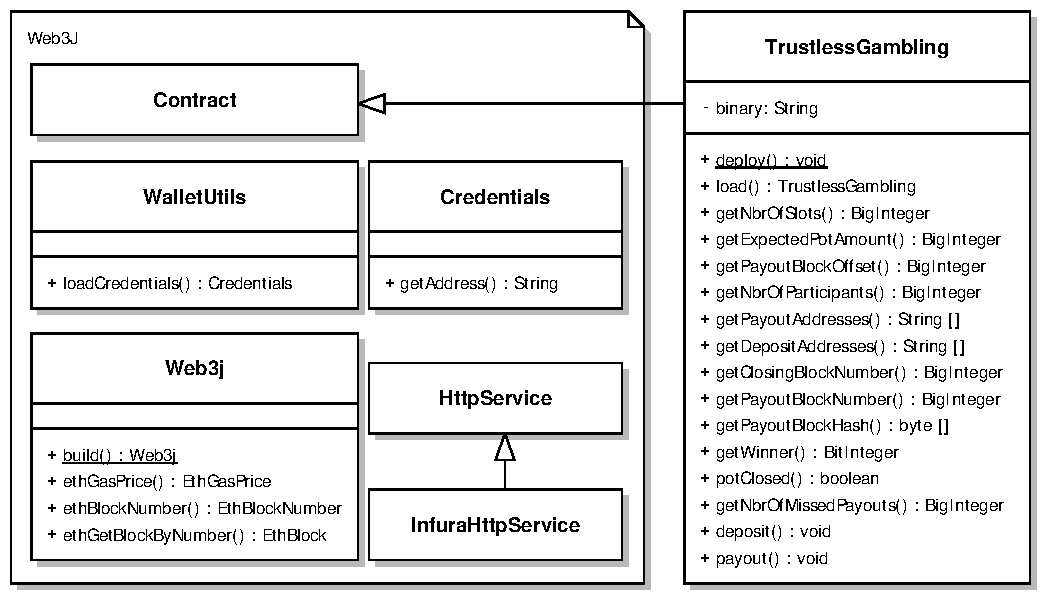
\includegraphics[width=1\linewidth]{Figures/umsetzung_eth/eth_web3j}
\decoRule
\caption{Klassendiagramm Web3J}
\label{fig:eth_web3j}
\end{figure}

Der folgende Java Code sorgt dafür, dass der von Web3J angesprochene Full Node den Smart Conrtact in einer Transaktion an das Rinkeby Testnetz sendet.

\begin{lstlisting}[basicstyle=\small]
public void createContract() throws Exception {
  String WALLET_FILENAME = "ethereum.json";
  String WALLET_PASSWORD = "changeit";
  long GAS_LIMIT = 1000000;
  ClassLoader classLoader = getClass().getClassLoader();
  File walletFile = new File(classLoader.getResource(WALLET_FILENAME).getFile());
  Credentials credentials = WalletUtils.loadCredentials(WALLET_PASSWORD, walletFile.getAbsolutePath());
  System.out.println("Account address = " + credentials.getAddress());
  Web3j web3j = Web3j.build(new InfuraHttpService("https://rinkeby.infura.io/" + UserConfiguration.API_KEY));
  BigInteger currentGasPrice = web3j.ethGasPrice().send().getGasPrice();
  TrustlessGambling contract = TrustlessGambling.deploy(web3j, credentials, currentGasPrice, BigInteger.valueOf(GAS_LIMIT)).send();
  String status = contract.getTransactionReceipt().get().getStatus();
  if ("0x1".equals(status)) {
    String address = contract.getContractAddress();
    System.out.println("Contract address = " + address);
    System.out.println("TXN hash = " + contract.getTransactionReceipt().get().getTransactionHash());
    System.out.println("Gas used = " + contract.getTransactionReceipt().get().getGasUsed());
  } else {
    System.out.println("Smart contract could not be deployed.");
  }
}
\end{lstlisting}

In Zeile 5 wird der Web3J Service erzeugt. Dieser kümmert sich um die Kommunikation mit dem Full Node. Die übergebene URL legt die Adresse des Full Nodes fest. Infura\footnote{\url{https://infura.io/}} ist dabei ein Service der sich auf das Hosting von Ethereum Full Nodes spezialisiert hat. Über einen API Schlüssel kann man sich zu seinem Full Node verbinden. Statt des von Infura betriebenen Nodes kann man auch einen eigens betriebenen Full Node verwenden, um die volle Kontrolle zu behalten. In diesem Fall verwendet man statt des \code{InfuraHttpService} direkt die Oberklasse \code{HttpService}.
Zeile 6 fragt den Full Node nach dem aktuell zu bezahlenden Gaspreis.
In Zeile 8 wird das durch die Web3J Comandline Tools erzeugte Wallet geladen. Mithilfe dieses wird unter Zuhilfenahme des Passworts die im nächsten Schritt verwendeten \code{Credentials} geladen.
In Zeile 11 wird der Smart Contract durch den Aufruf der statischen \code{TrustlessGambling.deploy} Methode in der Transaktion an das Netzwerk gesendet. Dabei wird ein Gaslimit von einer Million WEI festgelegt.
Die Ausführung des oben gezeigten Java Codes führt zu der folgenden Ausgabe:

\begin{lstlisting}[basicstyle=\small]
Account address = 0x2201f3919589b519135ce977cc0906c9481069b2
Contract address = 0x25c3136145fbd7f3b9217e58e2fabe3eb1928705
TXN hash = 0x06dce3c460b4caa595c5cc0f81ac78e7c70eeb1e89d3e0e6a017ea88e60dbce1
Gas used = 825846
\end{lstlisting}

Das Gaslimit von einer Million WEI hat ausgereicht und der Smart Contract befindet sich nun in der Blockchain des Ethereum Rinkeby Testnetzes. In einem Blockchain Explorer kann man die Details der vom Full Node erstellten Transaktion\footnote{\url{https://rinkeby.etherscan.io/tx/0x06dce3c460b4caa595c5cc0f81ac78e7c70eeb1e89d3e0e6a017ea88e60dbce1}} und den kompilierten Contract Code\footnote{\url{https://rinkeby.etherscan.io/address/0x25c3136145fbd7f3b9217e58e2fabe3eb1928705\#code}} anschauen.
\if Alternativ zu Web3J lässt sich der Contract Code mithilfe des Ethereum Clients namens Mist\footnote{\url{https://github.com/ethereum/mist}} veröffentlichen.
\fi

\subsection{Geschäftslogik Glücksspielanwendung}

Die Glücksspielanwendung zeigt lediglich den aktuellen Zustand des Smart Contracts an. Die gesamte Geschäftslogik des Smart Contracts wird vom Etherem Netzwerk ausgeführt. Sollte die Glücksspielanwendung aufgrund technischer Fehler ausfallen, hat dies keinerlei Auswirkung auf das eigentliche Spiel. Die Geschäftslogik der Glücksspielanwendung fragt lediglich in regelmäßigen Abständen beim Full Node an, ob eine Änderung des Smart Contract Zustands stattgefunden hat. Abbildung \ref{fig:eth_business_logic1} liefert einen ersten Überblick über die dazu verwendeten Klassen.

\begin{figure}[H]
\centering
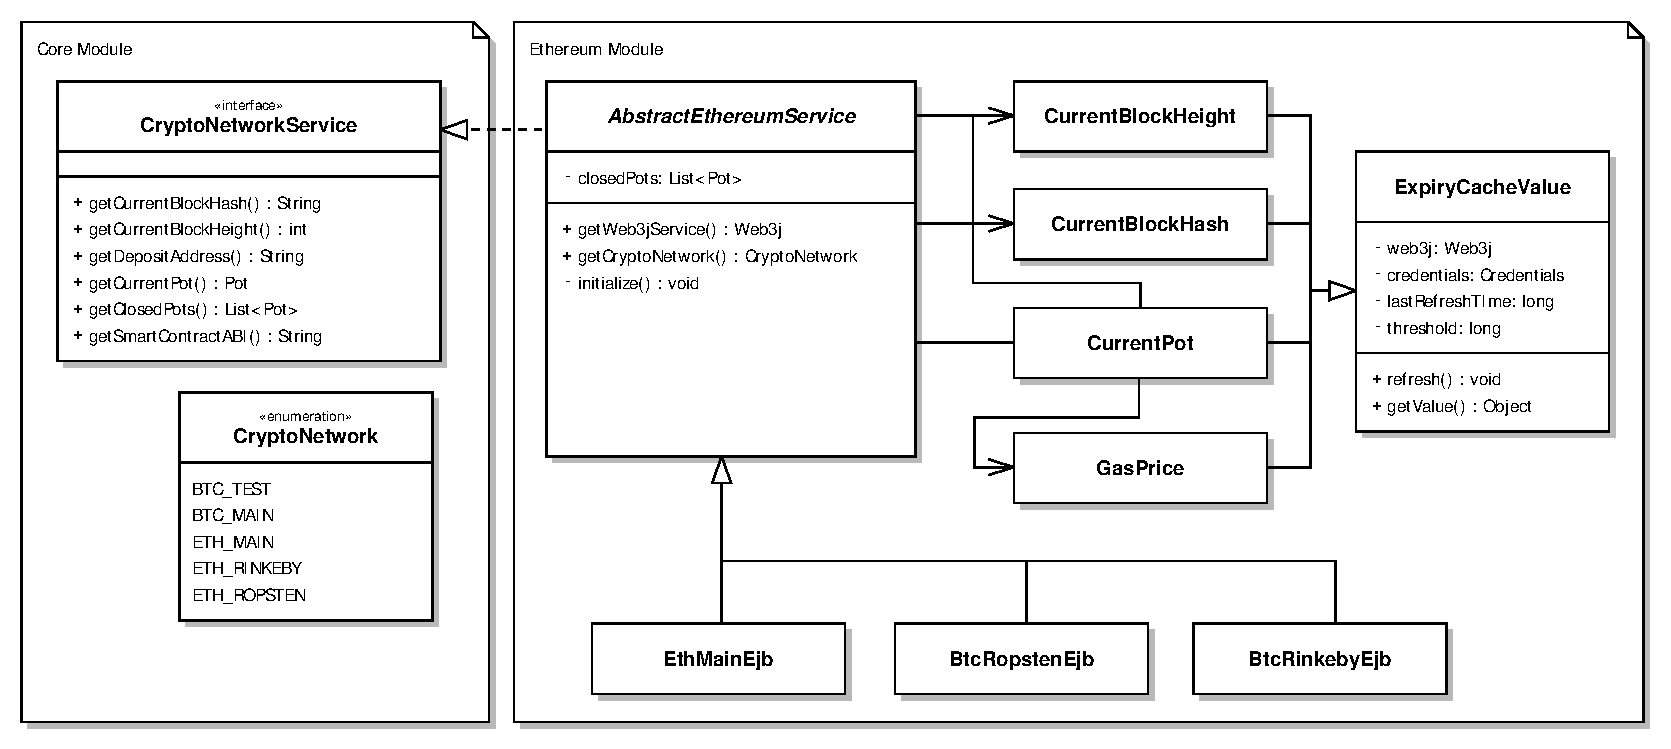
\includegraphics[width=1\linewidth]{Figures/umsetzung_eth/eth_business_logic1}
\decoRule
\caption{Klassendiagramm Ethereum}
\label{fig:eth_business_logic1}
\end{figure}

\subsubsection{Core Module}
Das \code{CryptoNetworkService} Interface wurde um die Methode \code{getSmartContractABI} erweitert. Bei dem  Smart Contract \textbf{A}pplication \textbf{B}inary \textbf{I}nterface handelt es sich um die statische zur Compile-Zeit bestimmte Schnittstellenbeschreibung, die festlegt wie man mit dem Smart Contract interagieren kann. Das Smart Contract ABI wird üblicherweise im JSON Format angegeben.

Zu dem \code{CryptoNetwork} Enum sind nun die zusätzlichen Werte \code{ETH\_MAIN, ETH\_RINKEBY, ETH\_ROPSTEN} hinzugekommen. Über diese Werte kann man steuern, mit welchem Ethereum Netzwerk die Anwendung kommunizieren soll. 
Die Klassen \code{Pot} und \code{Participant} haben sich nicht verändert.
\subsubsection{Ethereum Module: AbstractEthereumService}

Die abstrakte Klasse \code{AbstractEthereumService} implementiert die \code{CryptoNetworkService} Schnittstelle. Die Klassen \code{EthMainEjb, EthRopstenEjb und EthRinkebyEjb} legen lediglich über den verwendeten Web3J Service fest, welches Netzwerk die Anwendung ansprechen soll.
Die abstrakte Klasse \code{AbstractEthereumService} implementiert die vom \code{CryptoNetworkService} Interface geforderten Methoden. Die Methoden \code{getDepositAdress} und \code{getSmartContractABI} geben lediglich die statische Smart Contract Adresse und den Smart Contract ABI JSON String zurück. Die Methoden \code{getCurrentBlockHash, getCurrentBlockHeight} und \code{getCurrentPot} geben gecachte Werte des jeweiligen \code{ExpieryCacheValue} durch den Aufruf der \code{getValue} Methode an die Webanwendung zurück. Die Klassen \code{CurrentBlockHeight, CurrentBlockHash, GasPrice und CurrentPot} erweitern die abstrakte \code{ExpieryCacheValue} Klasse. Diese sorgt dafür, dass die Werte erst nach dem Ablauf einer gewissen konfigurierbaren Zeit (\code{threshold}) automatisch neu beim Full Node angefragt werden. Dies verhindert, dass der Full Node durch zu viele Anfragen überlastet wird. Alle Cache Werte werden in der \code{initialize} Methode der \code{AbstractEthereumService} Klasse initialisiert. 
\begin{lstlisting}[basicstyle=\small]
@PostConstruct
private void initialize() {
  log.info("#### start " + getClass().getSimpleName() + " network service ####");
  blockHightCache = new CurrentBlockHeight(getWeb3jService(), getCredentials());
  log.info("blockHight=" + blockHightCache.getValue().intValue());
  blockHashCache = new CurrentBlockHash(getWeb3jService(), getCredentials(), blockHightCache);
  log.info("blockHash=" + blockHashCache.getValue());
  gasPriceCache = new GasPrice(getWeb3jService(), getCredentials());
  log.info("gasPrice=" + gasPriceCache.getValue().intValue());
  currentPotCache = new CurrentPot(getWeb3jService(), getCredentials(), gasPriceCache, blockHightCache,
  		UserConfiguration.CONTRACT_ADDRESS);
  log.info("currentPot=" + currentPotCache.getValue().toString());
}
\end{lstlisting}



\subsubsection{Ethereum Module: CurrentBlockHash}

Der folgende Code zeigt beispielhaft die die Implementierung des \code{CurrentBlockHash ExpieryCacheValue}.

\begin{lstlisting}[basicstyle=\small]
public class CurrentBlockHash extends ExpiryCacheValue {

  CurrentBlockHeight blockHeight;

  public CurrentBlockHash(Web3j web3j, Credentials credentials, CurrentBlockHeight blockHeight) {
    super(web3j, credentials, 5 * SECOND);
    this.blockHeight = blockHeight;
  }

  /**
   * refresh if cache value expired. Called automatically by the ExpiryCacheValue.getValue()
   * method.
   */
  @Override
  protected void refresh() {
    String blockHash = fetchCurrentBlockHash();
    if (blockHash != null)
      setValue(blockHash);
  }

  private String fetchCurrentBlockHash() {
    String result = "error";
    DefaultBlockParameterNumber number = new DefaultBlockParameterNumber(blockHeight.getValue());;
    try {
      EthBlock ethBlock = getWeb3jService().ethGetBlockByNumber(number, false).send();
    result = ethBlock.getBlock().getHash();
    } catch (IOException e) {
      e.printStackTrace();
    }
    return result;
  }
}
\end{lstlisting}



In Zeile 6 wird konfiguriert, dass der aktuelle Blockhash maximal alle 5 Sekunden vom Full Node abgefragt wird. In Zeile 18 wird durch den Aufruf der \code{ethGetBlockByNumber} Methode der Block der aktuellen Blocknummer angefragt. Über den Wahrheitswertparameter kann man entweder die gesamten Blockdaten oder nur die Header-Informationen beim Full Node anfragen.

\subsubsection{Ethereum Module: CurrentBlockHeight}
Die Implementierung des \code{CurrentBlockHeight ExpieryCacheValue} greift auf die folgenden Zeilen Code zurück. Es findet maximal alle 5 Sekunden eine Anfrage an den Full Node statt.

\begin{lstlisting}[basicstyle=\small]
EthBlockNumber ethBlockNumber = getWeb3jService().ethBlockNumber().send();
BigInteger currentBlockNumber = ethBlockNumber.getBlockNumber();
\end{lstlisting}

\subsubsection{Ethereum Module: GasPrice}

Die Implementierung des \code{GasPrice ExpieryCacheValue} greift auf die folgenden Zeilen Code zurück. Es findet maximal alle 60 Sekunden eine Anfrage an den Full Node statt.

\begin{lstlisting}[basicstyle=\small]
EthGasPrice ethGasPrice = getWeb3jService().ethGasPrice().send();
BigInteger gasPrice = ethGasPrice.getGasPrice();
\end{lstlisting}


\subsubsection{Ethereum Module: CurrentPot}

Der \code{CurrentPot ExpieryCacheValue} verwendet die Klasse \code{TrustlessGambling} um den Zustand des Smart Contracts zu erfassen und in die Klasse \code{Pot} abzubilden. Im Konstruktor des \code{CurrentPot ExpieryCacheValue} wird die Methode \code{createEmptyPot} aufgerufen.

\begin{lstlisting}[basicstyle=\small]
private Pot createEmptyPot() throws Exception{
    TrustlessGambling contract = TrustlessGambling.load(contractAddress, getWeb3jService(),
            getCredentials(), gasPrice.getValue(), BigInteger.valueOf(5300000));
    int nbrOfSlots = contract.NBR_OF_SLOTS().send().intValue();
    long amount = contract.EXPECTED_POT_AMOUNT().send().longValue();
    return new Pot(nbrOfSlots, amount);
}
\end{lstlisting}



Diese Methode fragt den Full Node, wie viele Spieler und welcher Einzahlungsbetrag vom Smart Contract erwartet wird und erzeugt anschließend einen neuen leeren Topf. Der Zustand des Topfs wird durch den folgenden Code jedes mal aktualisiert, wenn die \code{refresh} Methode des \code{ExpieryCacheValue} aufgerufen wird. Dies findet alle 10 Sekunden statt.

\input{CodeSnippets/eth/currentPot.tex}

Der Code unterscheidet zwischen der Anzahl der Teilnehmer, die die Glücksspielanwendung lokal zwischenspeichert(Zeile 4) und der Anzahl Teilnehmer des Datenfeldes des Smart Contracts (Zeile 5). Wenn neue Teilnehmer durch den Aufruf der \code{deposit} Methode in den Smart Contract einzahlen, wird der Topf durch die Zeilen 7 bis 11 aktualisiert. Die Ein- und Auszahlungsadressen der neuen Teilnehmer werden dazu aus den Smart Conract Daten geladen.
Durch die letzte Einzahlung wechselt der Smart Contract in den Status \code{closed}. Ab diesem Moment wird der Topf durch die Abarbeitung des Codes ab Zeile 30 aktualisiert. Zunächst werden die finalen \code{closingBlockNumber} und \code{payoutBlockNumber} Werte aus den Smart Contract Daten geladen und die \code{currentBlockNumber} durch den Full Node bestimmt. Anschließend wird zwischen 3 Fällen unterschieden:
\begin{enumerate}
\item Zeile 38: Der zur Gewinnerauswahl benötigte Block wurde noch nicht gefunden. Dies bedeutet, dass ein Aufruf der \code{payout} Methode des Smart Contracts noch nicht möglich ist.
\item Zeile 43: Der zur Gewinnerauswahl benötigte Block wurde gefunden und die \code{payout} Methode kann aufgerufen werden. In diesem Fall wird dem Benutzer angezeigt, wie viel Zeit er noch für den Aufruf der \code{payout} Methode hat. 
\item Zeile 46: Der zur Gewinnerauswahl benötigte Block wurde zwar gefunden, es sind allerdings bereits mehr als 256 Blöcke zwischen der letzten Einzahlung und dem aktuellen Zeitpunkt vergangen. Der Smart Contract wird bei dem Aufruf der \code{payout} Methode nicht auf den Blockhash für die Gewinnerauswahl zugreifen können. Der Gewinn wird zum nächsten Topf hinzufügen.
\end{enumerate}
Durch den Aufruf der \code{payout} Methode wird das Datenfeld, das die Anzahl der aktuellen Teilnehmer des Smart Contracts speichert, auf den Wert Null gesetzt. Da der lokal gespeicherte Topf aber noch alle Teilnehmer enthält, hat dies zur Folge, dass beim erneuten Aufruf der \code{refresh} Methode des \code{CurrenPot ExpieryCacheValue} die Bedingung aus Zeile 6 verletzt ist und der Code von Zeile 13 bis 27 ausgeführt wird. Diese Codezeilen laden den Gewinner und den \code{payoutBlockHash} aus den Daten des Smart Contracts. Hat der \code{payoutBlockHash} den Wert Null, wurde die \code{payout} Methode zu spät aufgerufen. Nur in diesem Fall gibt es keinen Gewinner. Anschließend wird der aktuelle Topf zur Liste der abgearbeiteten Töpfe hinzugefügt und ein neuer Topf durch den Aufruf der \code{createEmptyPot} Methode erzeugt.

\subsection{Grafische Benutzeroberfläche}

Das folgende Beispiel betrachtet einen frisch auf dem Ethereum Rinkeby Testnetzwerk bereitgestellten Smart Contract.

\begin{figure}[H]
\centering
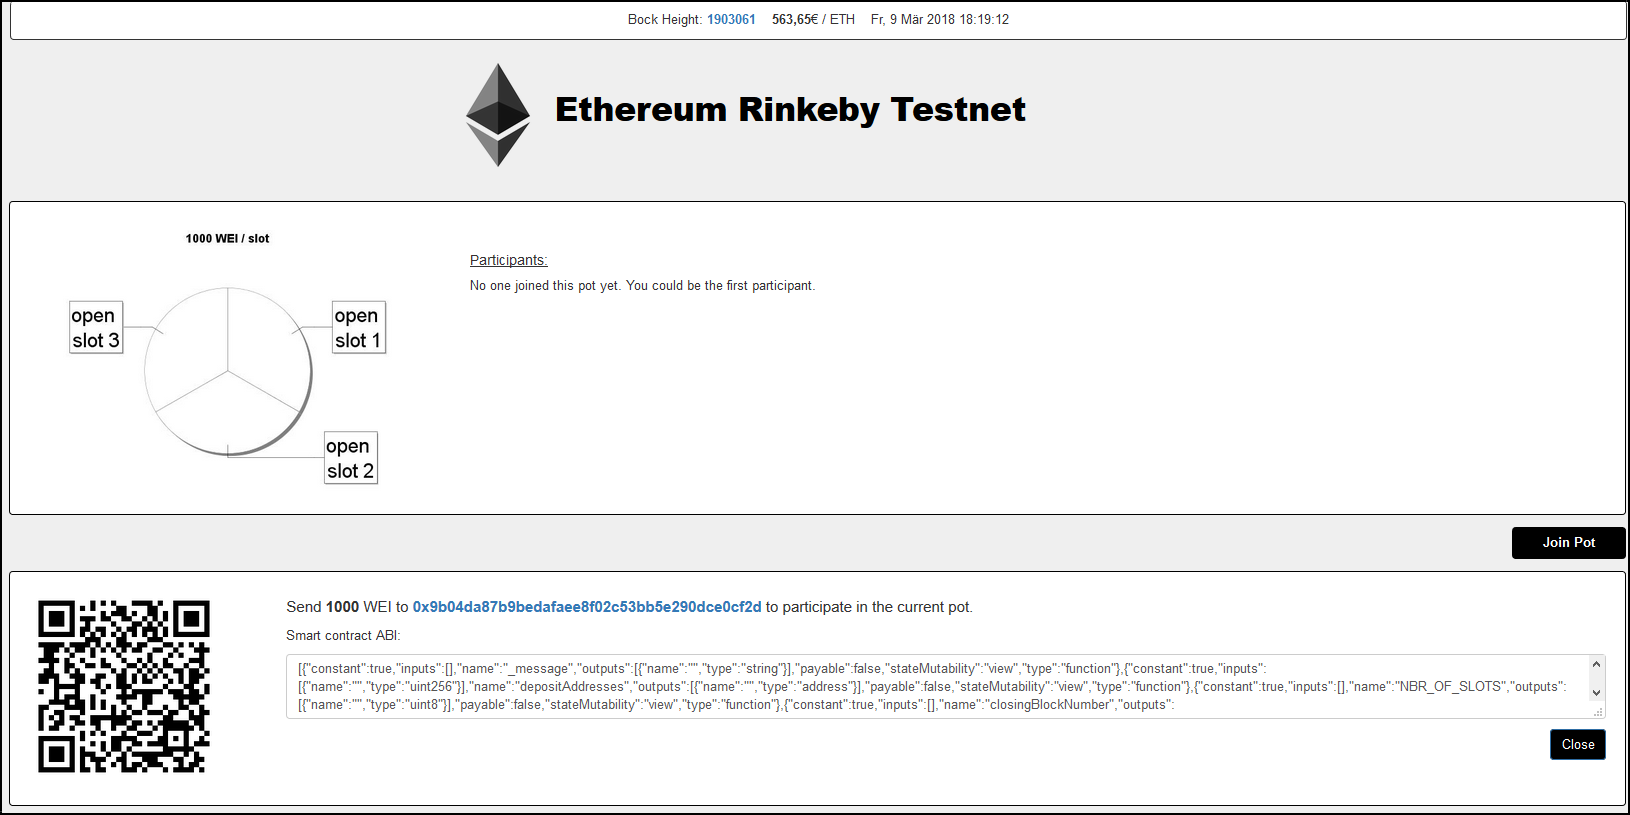
\includegraphics[width=1\linewidth]{Figures/eth_gui/ETH_pot_empty}
\decoRule
\caption{Leerer Topf}
\label{fig:ETH_pot_empty}
\end{figure}
Abbildung \ref{fig:ETH_pot_empty} zeigt einen Topf mit 3 freien Plätzen. Um dem Spiel beizutreten, muss der Spieler den Betrag von 1000 WEI an den Smart Contract senden. Genau wie bei Bitcoin wird dem Nutzer ein QR-Code angezeigt, der die Übermittlung der Daten in einen Smartphone Client erleichtert. Das \textbf{E}thereum \textbf{I}mprovement \textbf{P}roposal Nummer 681\cite{eip681} legt die Kodierung der Daten fest.
Folgende Daten sind in dem QR Code enthalten:\\ ''ethereum:0x9b04da87b9bedafaee8f02c53bb5e290dce0cf2d/deposit?value=1000''. In diesem Beispiel verwenden wir für die Interaktion mit dem Netzwerk keinen Smartphone Client sondern die Webanwendung namens ''My Ether Wallet''\footnote{\url{https://www.myetherwallet.com/\#contracts}}. Diese benötigt für die Interaktion mit dem Smart Contract sowohl die Contract Adresse als auch das \textbf{A}pplication \textbf{B}inary \textbf{I}nterface.


\begin{figure}[H]
\centering
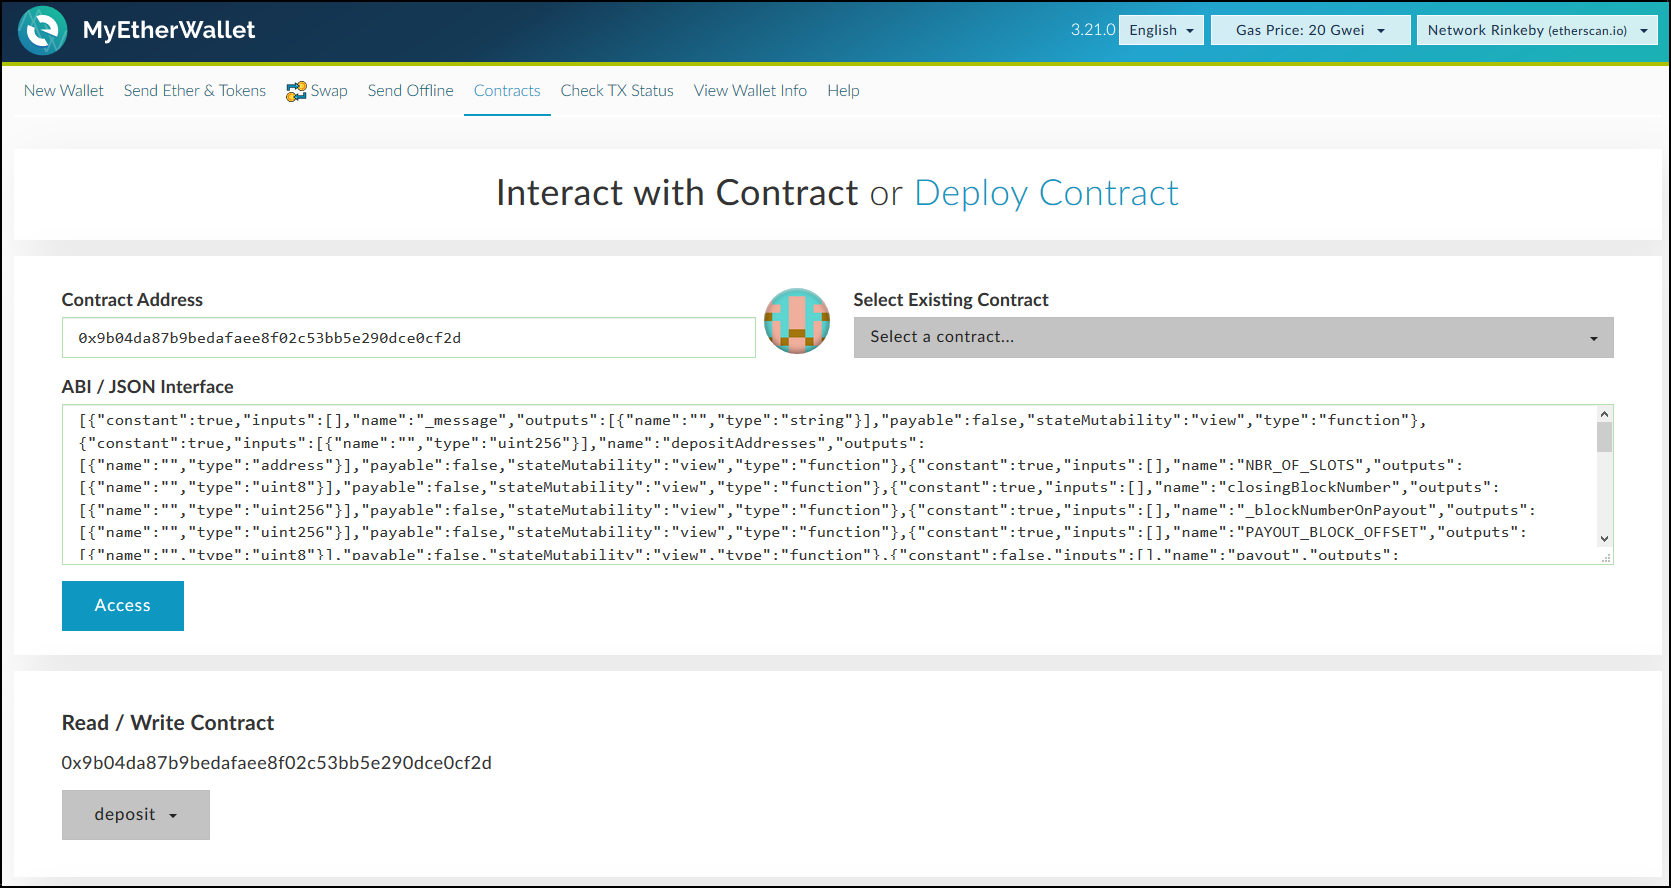
\includegraphics[width=1\linewidth]{Figures/eth_gui/ETH_wallet}
\decoRule
\caption{My Ether Wallet}
\label{fig:ETH_wallet}
\end{figure}

Nachdem der Nutzer diese wie in Abbildung \ref{fig:ETH_wallet} eingegeben hat, kann er über eine Dropdown-Liste die gewünschte Funktion des Smart Contracts aufrufen.


\begin{figure}[H]
\centering
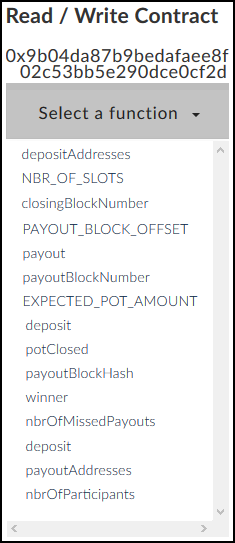
\includegraphics[scale=0.85]{Figures/eth_gui/ETH_wallet_contract_functions}
\decoRule
\caption{Liste aller Smart Contract Funktionen}
\label{fig:ETH_wallet_contract_functions}
\end{figure}

Abbildung \ref{fig:ETH_wallet_expected_amount} zeigt den Aufruf der Funktion auf, die zurückgibt, welchen Geldbetrag der Smart Contract vom Spieler erwartet.

\begin{figure}[H]
\centering
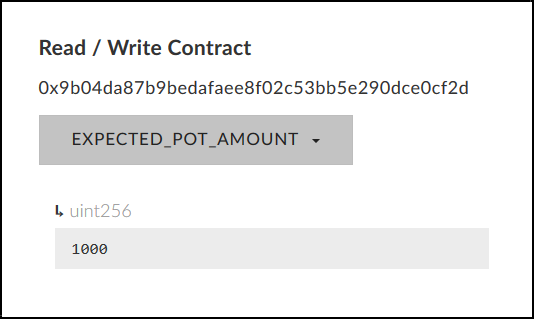
\includegraphics[scale=0.85]{Figures/eth_gui/ETH_wallet_expected_amount}
\decoRule
\caption{Aufruf der \code{EXPECTED\_POT\_AMOUNT} Funktion}
\label{fig:ETH_wallet_expected_amount}
\end{figure}

Da es sich lediglich um einen lesenden Zugriff handelt, wird keine Transaktion ans Netzwerk gesendet, beziehungsweise in die Blockchain geschrieben. Es fallen somit keine Transaktionskosten an.

\begin{figure}[H]
\centering
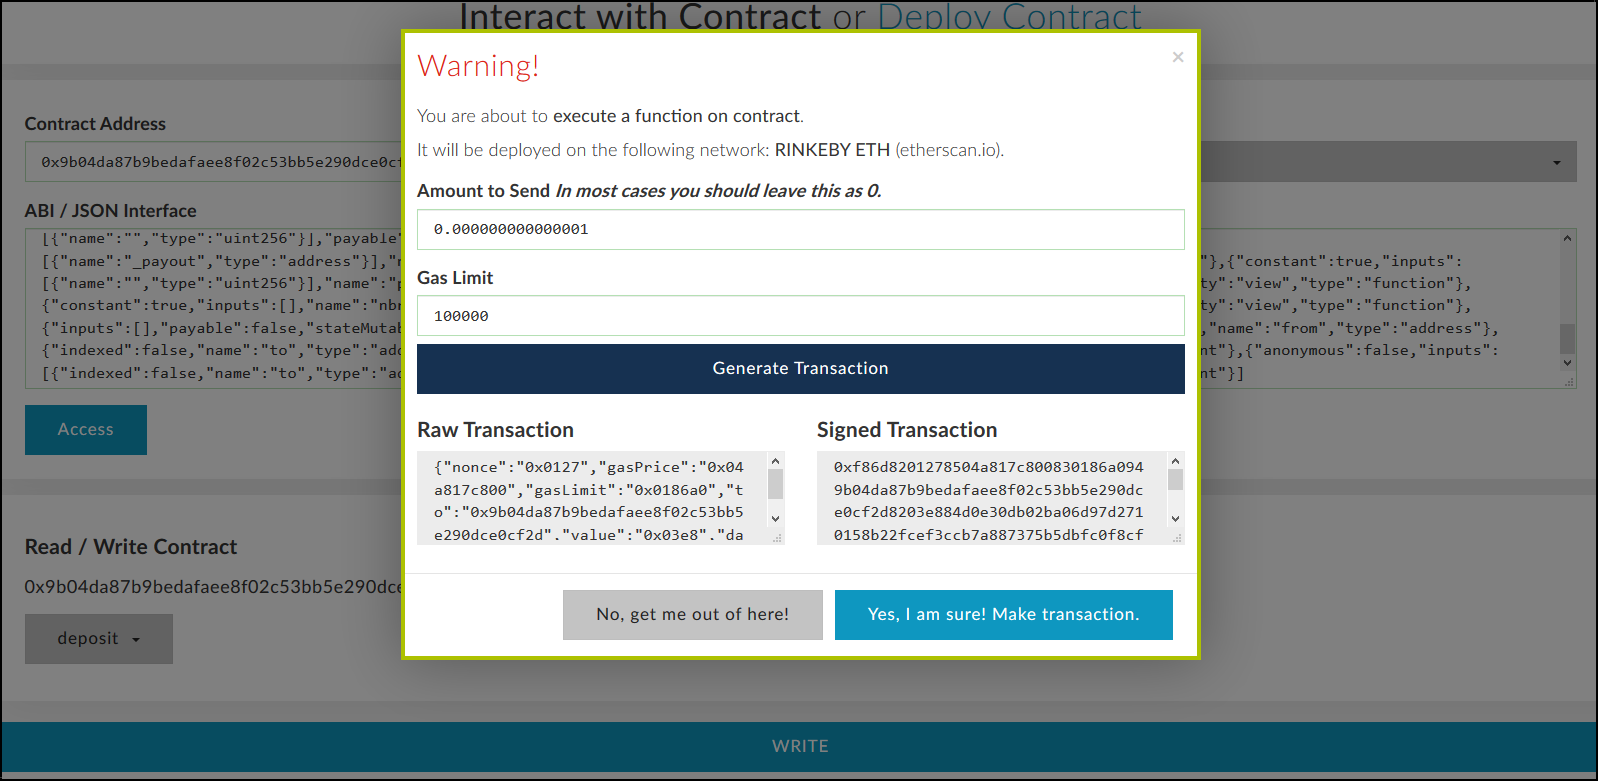
\includegraphics[width=1\linewidth]{Figures/eth_gui/ETH_wallet_deposit}
\decoRule
\caption{Aufruf der \code{deposit} Funktion}
\label{fig:ETH_wallet_deposit}
\end{figure}

Da der Nutzer nun nachgeprüft hat, dass der Smart Contract wirklich Zahlungen von 1000 WEI erwartet, kann er die \code{depsoit} Funktion mit diesem Betrag aufrufen.
Die Wallet Webseite erwartet den Betrag in der Einheit Ether. Die geforderten 1000 WEI entsprechen 0.000000000000001 Ether. Die Umrechnung kann der Spieler mittels eines Online Konverters\footnote{\url{https://etherconverter.online/}} durchführen.
Nun muss die erstellte Transaktion nur noch signiert werden. Der Nutzer kann der Webseite dazu seinen privaten Schlüssel mitteilen oder die Signierung eigenständig durch ein sogenanntes Hardware Wallet durchführen. Die Herausgabe seines privaten Schlüssels an eine Webseite ist aus sicherheitstechnischer Sicht keine gute Praktik. Sollte der Webseitenbetreiber böse Absichten haben oder die Webseite gehackt werden, führt dies zum Verlust des durch den Schlüssel kontrollierten Geldes. Eine sichere Variante ist die Verwendung eines Hardware Wallets. Dieses speichert alle privaten Schlüssel und führt die Signatur eigenständig durch. Der verwendete private Schlüssel verlässt somit niemals das Gerät. 

\begin{figure}[H]
\centering
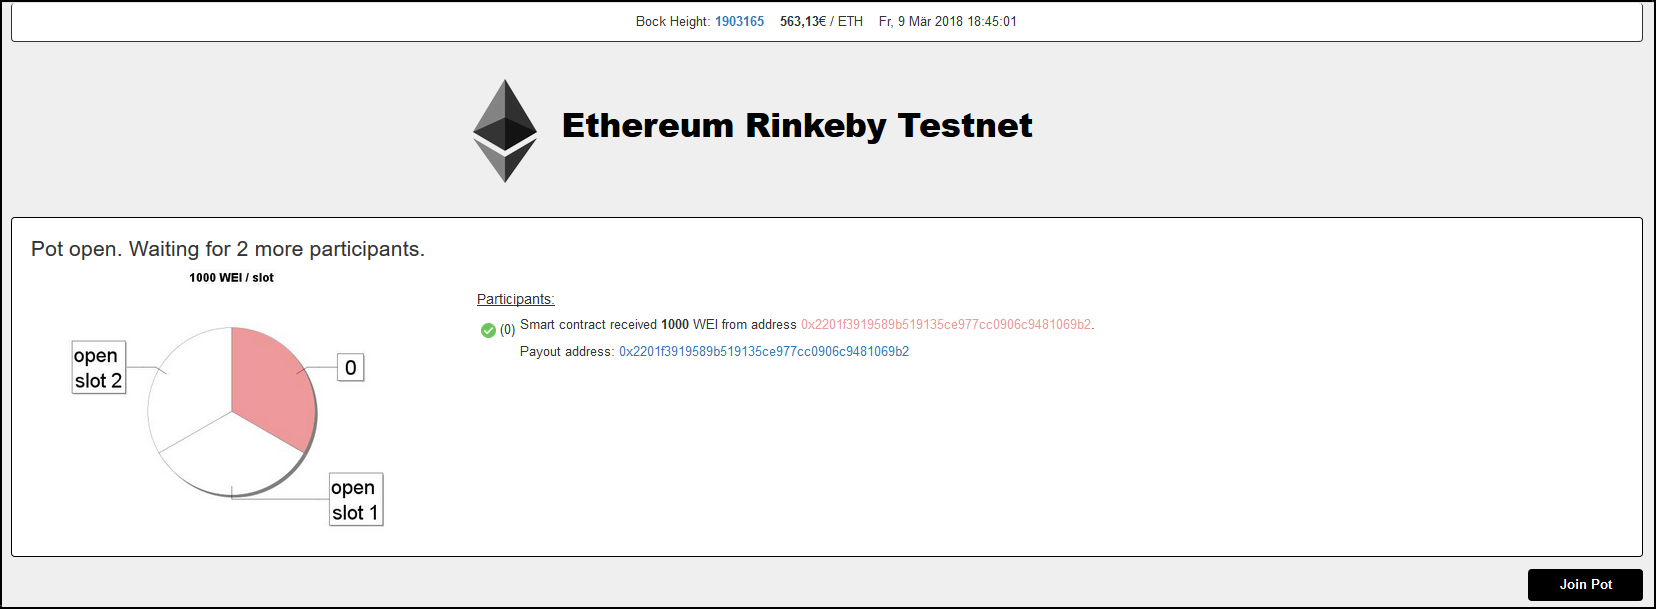
\includegraphics[width=1\linewidth]{Figures/eth_gui/ETH_pot_1}
\decoRule
\caption{Eingang der ersten Zahlung}
\label{fig:ETH_pot_1}
\end{figure}

Abbildung \ref{fig:ETH_pot_1} visualisiert den Zustand des Smart Contracts nachdem die erste Einzahlungstransaktion in die Blockchain aufgenommen wurde.

\begin{figure}[H]
\centering
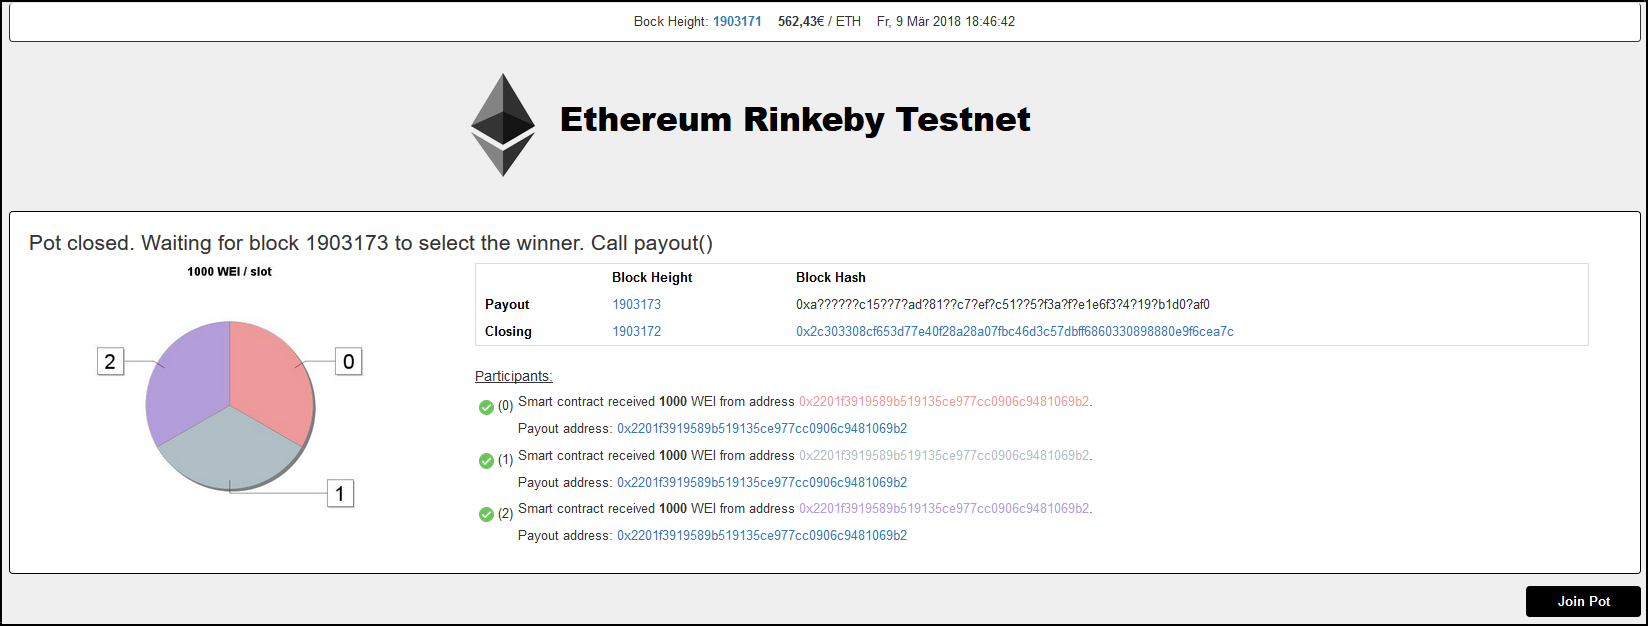
\includegraphics[width=1\linewidth]{Figures/eth_gui/ETH_pot_closed}
\decoRule
\caption{Topf geschlossen}
\label{fig:ETH_pot_closed}
\end{figure}

Abbildung \ref{fig:ETH_pot_closed} visualisiert den Zustand des Smart Contracts nachdem die letzte Einzahlungstransaktion in die Blockchain aufgenommen wurde. Der Smart Contract hat den Topf geschlossen und wartet nun, dass einer der Spieler die \code{payout} Funktion aufruft.

\begin{figure}[H]
\centering
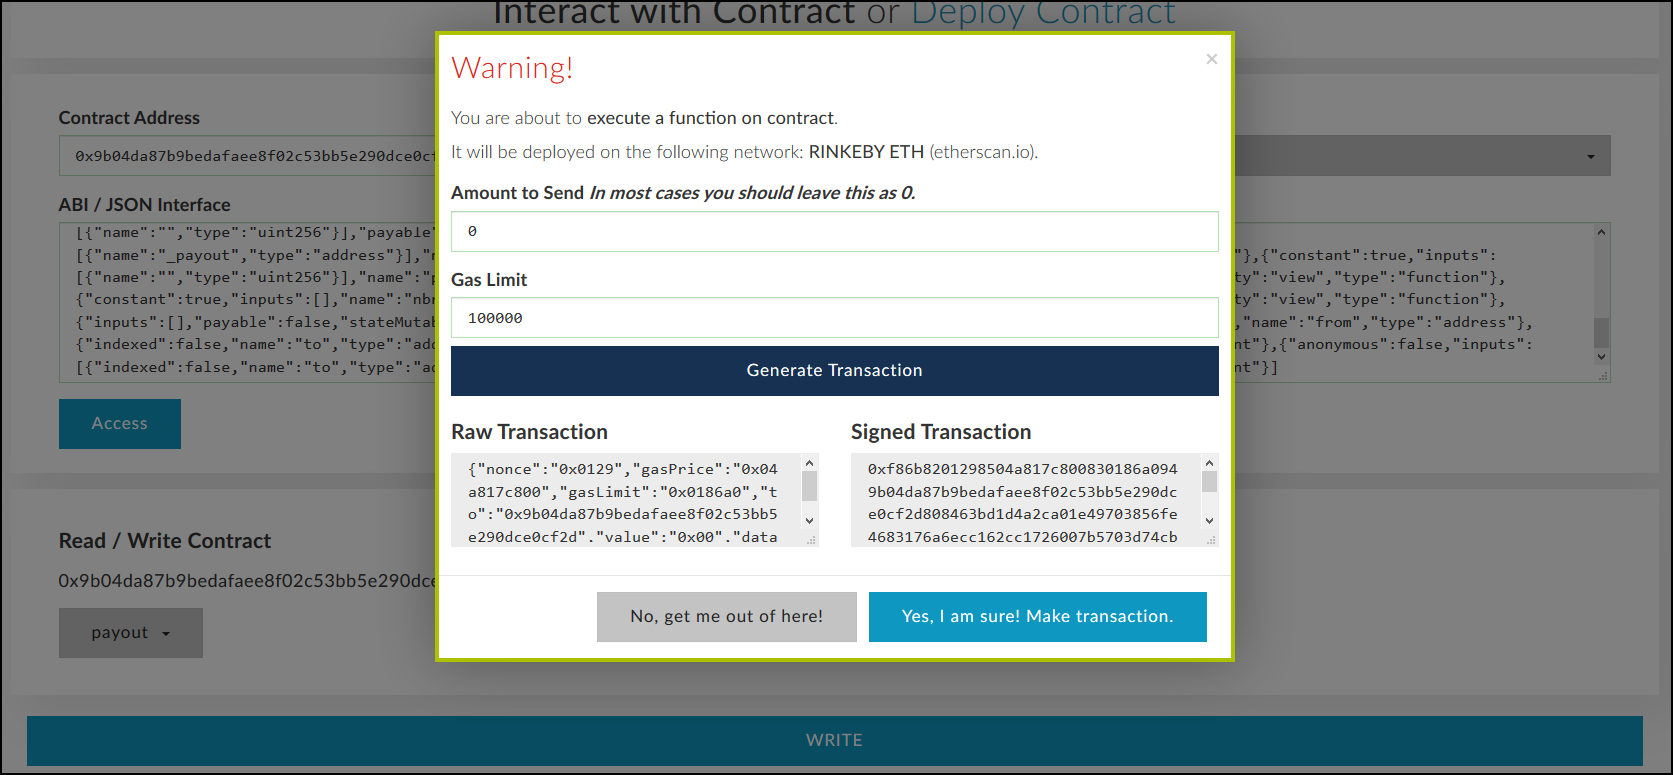
\includegraphics[width=1\linewidth]{Figures/eth_gui/ETH_wallet_payout}
\decoRule
\caption{Aufruf der \code{payout} Funktion}
\label{fig:ETH_wallet_payout}
\end{figure}

In Abbildung \ref{fig:ETH_wallet_payout} ist gezeigt wie ein Spieler die  \code{payout} Funktion aufruft. Durch den Aufruf dieser Funktion wird der Gewinner ausgewählt, die Auszahlung getätigt und der Topf wieder geöffnet.

\begin{figure}[H]
\centering
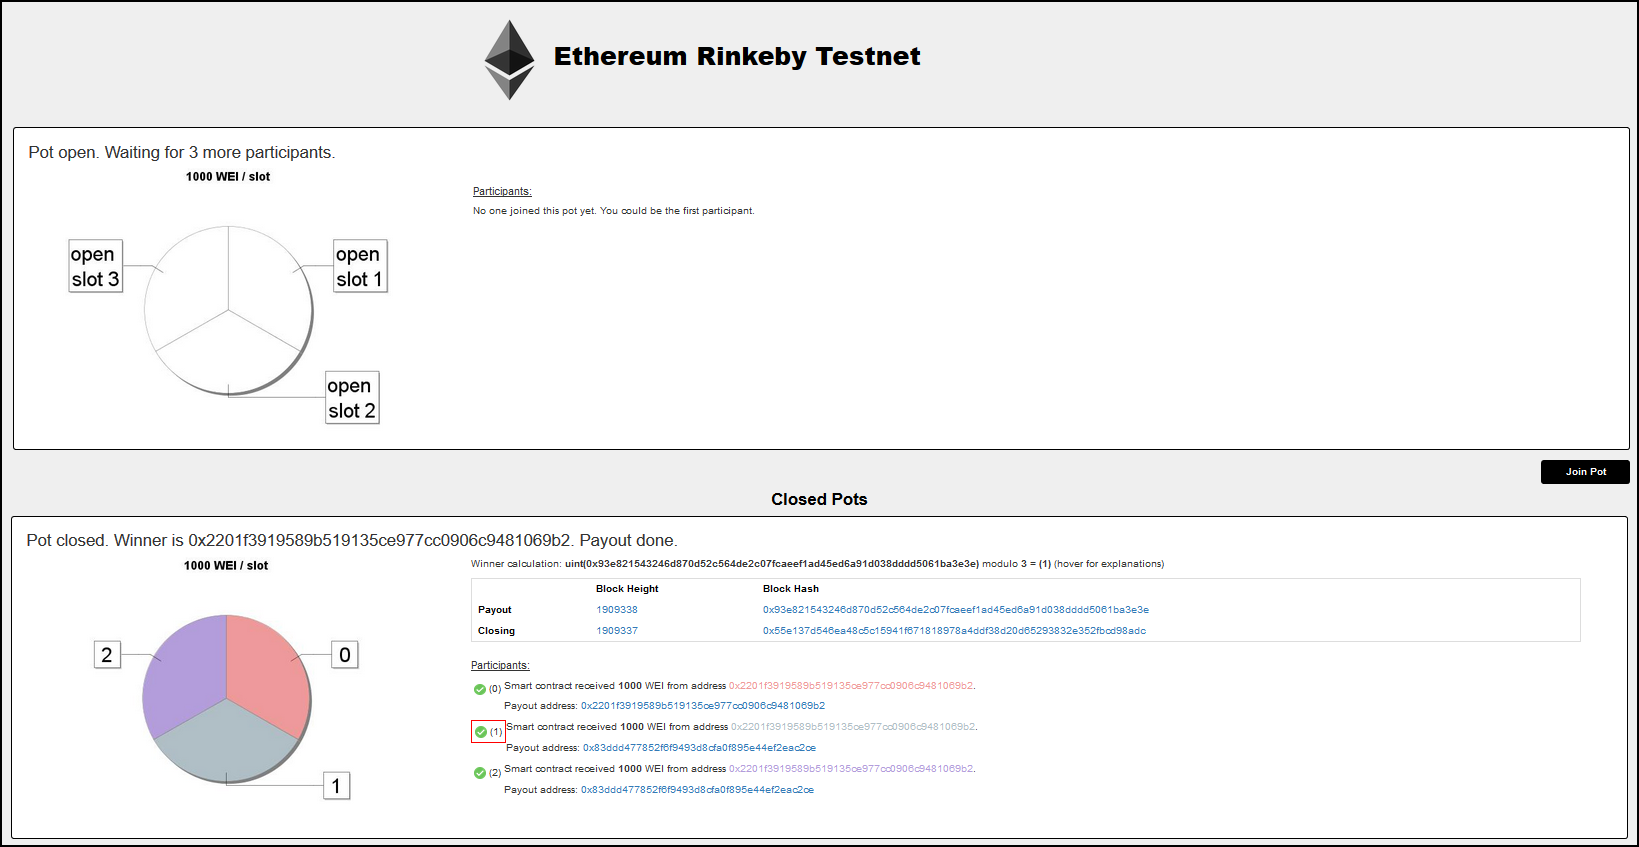
\includegraphics[width=1\linewidth]{Figures/eth_gui/ETH_pot_finished}
\decoRule
\caption{Gewinner ausgewählt}
\label{fig:ETH_pot_finished}
\end{figure}

Abbildung \ref{fig:ETH_pot_finished} zeigt den Gewinner des alten Topfs und den neu geöffneten Topf.

\begin{figure}[H]
\centering
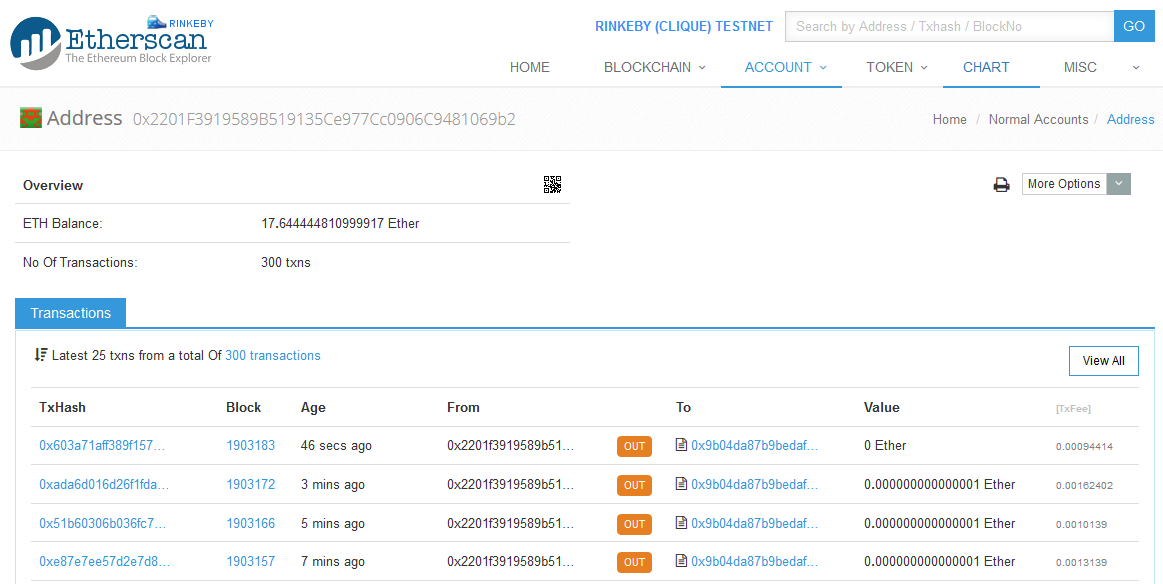
\includegraphics[width=1\linewidth]{Figures/eth_gui/contract_transactions}
\decoRule
\caption{Block Explorer: Smart Contract}
\label{fig:contract_transactions}
\end{figure}

Abbildung \ref{fig:contract_transactions} zeigt die 3 Einzahlungstransaktionen und die Transaktion, die die \code{payout} Funktion aufruft.

\begin{figure}[H]
\centering
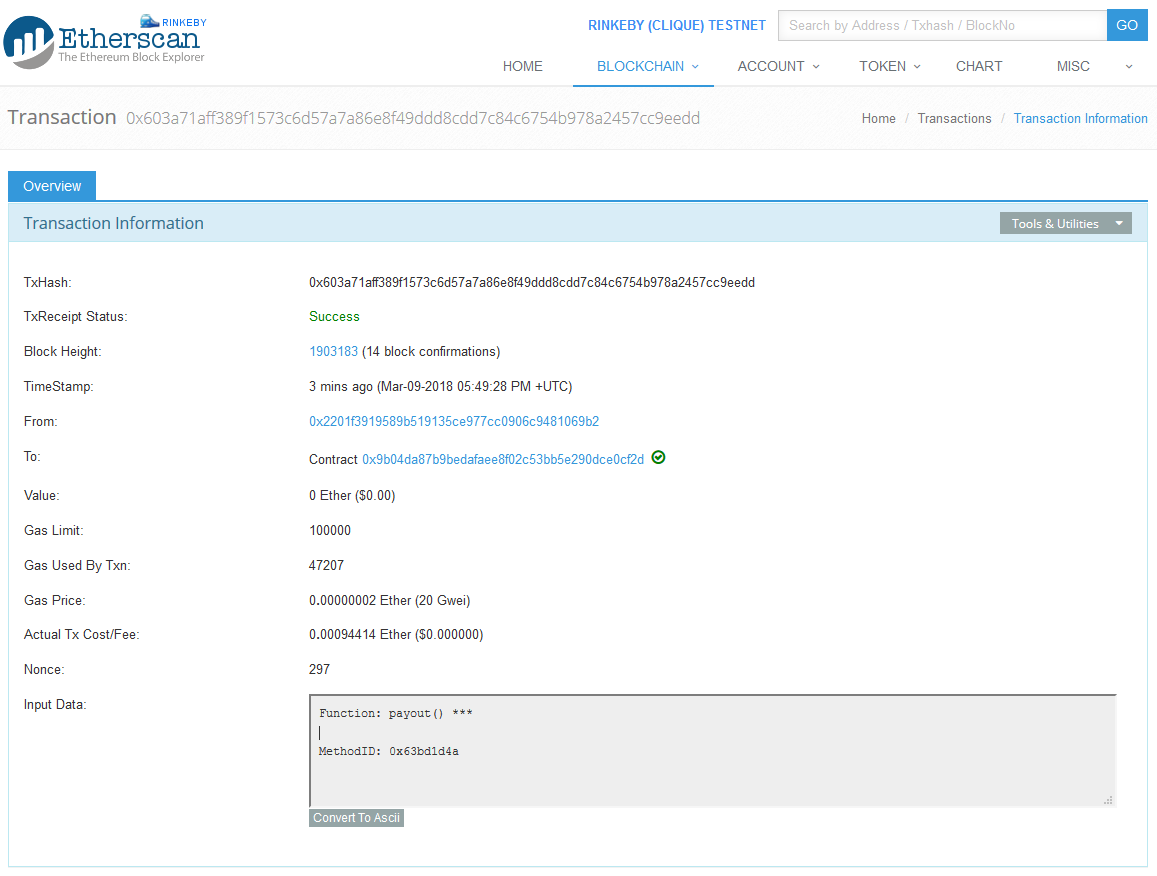
\includegraphics[width=1\linewidth]{Figures/eth_gui/contract_payout_txn}
\decoRule
\caption{Block Explorer: Payout Transaktion}
\label{fig:contract_payout_txn}
\end{figure}

Abbildung \ref{fig:contract_transactions} zeigt die Details der Transaktion, die die \code{payout} Funktion aufruft.